
\documentclass[journal,12pt,twocolumn]{IEEEtran}
%
\usepackage{setspace}
\usepackage{gensymb}
\usepackage{xcolor}
\usepackage{caption}
%\usepackage{subcaption}
%\doublespacing
\singlespacing

%\usepackage{graphicx}
%\usepackage{amssymb}
%\usepackage{relsize}
\usepackage[cmex10]{amsmath}
\usepackage{mathtools}
%\usepackage{amsthm}
%\interdisplaylinepenalty=2500
%\savesymbol{iint}
%\usepackage{txfonts}
%\restoresymbol{TXF}{iint}
%\usepackage{wasysym}
\usepackage{hyperref}
\usepackage{amsthm}
\usepackage{mathrsfs}
\usepackage{txfonts}
\usepackage{stfloats}
\usepackage{cite}
\usepackage{cases}
\usepackage{subfig}
%\usepackage{xtab}
\usepackage{longtable}
\usepackage{multirow}
%\usepackage{algorithm}
%\usepackage{algpseudocode}
%\usepackage{enumerate}
\usepackage{enumitem}
\usepackage{mathtools}
%\usepackage{iithtlc}
%\usepackage[framemethod=tikz]{mdframed}
\usepackage{listings}
\usepackage{tikz}
\usetikzlibrary { decorations.pathmorphing, decorations.pathreplacing, decorations.shapes, }
\let\vec\mathbf


%\usepackage{stmaryrd}


%\usepackage{wasysym}
%\newcounter{MYtempeqncnt}
\DeclareMathOperator*{\Res}{Res}
%\renewcommand{\baselinestretch}{2}
\renewcommand\thesection{\arabic{section}}
\renewcommand\thesubsection{\thesection.\arabic{subsection}}
\renewcommand\thesubsubsection{\thesubsection.\arabic{subsubsection}}

\renewcommand\thesectiondis{\arabic{section}}
\renewcommand\thesubsectiondis{\thesectiondis.\arabic{subsection}}
\renewcommand\thesubsubsectiondis{\thesubsectiondis.\arabic{subsubsection}}

%\renewcommand{\labelenumi}{\textbf{\theenumi}}
%\renewcommand{\theenumi}{P.\arabic{enumi}}

% correct bad hyphenation here
\hyphenation{op-tical net-works semi-conduc-tor}

\lstset{
language=Python,
frame=single, 
breaklines=true,
columns=fullflexible
}



\begin{document}
%

\theoremstyle{definition}
\newtheorem{theorem}{Theorem}[section]
\newtheorem{problem}{Problem}
\newtheorem{proposition}{Proposition}[section]
\newtheorem{lemma}{Lemma}[section]
\newtheorem{corollary}[theorem]{Corollary}
\newtheorem{example}{Example}[section]
\newtheorem{definition}{Definition}[section]
%\newtheorem{algorithm}{Algorithm}[section]
%\newtheorem{cor}{Corollary}
\newcommand{\BEQA}{\begin{eqnarray}}
\newcommand{\EEQA}{\end{eqnarray}}
\newcommand{\define}{\stackrel{\triangle}{=}}
\newcommand{\myvec}[1]{\ensuremath{\begin{pmatrix}#1\end{pmatrix}}}
\newcommand{\mydet}[1]{\ensuremath{\begin{vmatrix}#1\end{vmatrix}}}

\bibliographystyle{IEEEtran}
%\bibliographystyle{ieeetr}

\providecommand{\nCr}[2]{\,^{#1}C_{#2}} % nCr
\providecommand{\nPr}[2]{\,^{#1}P_{#2}} % nPr
\providecommand{\mbf}{\mathbf}
\providecommand{\pr}[1]{\ensuremath{\Pr\left(#1\right)}}
\providecommand{\qfunc}[1]{\ensuremath{Q\left(#1\right)}}
\providecommand{\sbrak}[1]{\ensuremath{{}\left[#1\right]}}
\providecommand{\lsbrak}[1]{\ensuremath{{}\left[#1\right.}}
\providecommand{\rsbrak}[1]{\ensuremath{{}\left.#1\right]}}
\providecommand{\brak}[1]{\ensuremath{\left(#1\right)}}
\providecommand{\lbrak}[1]{\ensuremath{\left(#1\right.}}
\providecommand{\rbrak}[1]{\ensuremath{\left.#1\right)}}
\providecommand{\cbrak}[1]{\ensuremath{\left\{#1\right\}}}
\providecommand{\lcbrak}[1]{\ensuremath{\left\{#1\right.}}
\providecommand{\rcbrak}[1]{\ensuremath{\left.#1\right\}}}
\theoremstyle{remark}
\newtheorem{rem}{Remark}
\newcommand{\sgn}{\mathop{\mathrm{sgn}}}
\providecommand{\abs}[1]{\left\vert#1\right\vert}
\providecommand{\res}[1]{\Res\displaylimits_{#1}} 
\providecommand{\norm}[1]{\lVert#1\rVert}
\providecommand{\mtx}[1]{\mathbf{#1}}
\providecommand{\mean}[1]{E\left[ #1 \right]}
\providecommand{\fourier}{\overset{\mathcal{F}}{ \rightleftharpoons}}
\providecommand{\ztrans}{\overset{\mathcal{Z}}{ \rightleftharpoons}}

%\providecommand{\hilbert}{\overset{\mathcal{H}}{ \rightleftharpoons}}
\providecommand{\system}{\overset{\mathcal{H}}{ \longleftrightarrow}}
	%\newcommand{\solution}[2]{\textbf{Solution:}{#1}}
\newcommand{\solution}{\noindent \textbf{Solution: }}
\providecommand{\dec}[2]{\ensuremath{\overset{#1}{\underset{#2}{\gtrless}}}}
\numberwithin{equation}{section}
%\numberwithin{equation}{subsection}
%\numberwithin{problem}{subsection}
%\numberwithin{definition}{subsection}
\makeatletter
\@addtoreset{figure}{problem}
\makeatother

\let\StandardTheFigure\thefigure
%\renewcommand{\thefigure}{\theproblem.\arabic{figure}}
\renewcommand{\thefigure}{\theproblem}


%\numberwithin{figure}{subsection}

\def\putbox#1#2#3{\makebox[0in][l]{\makebox[#1][l]{}\raisebox{\baselineskip}[0in][0in]{\raisebox{#2}[0in][0in]{#3}}}}
     \def\rightbox#1{\makebox[0in][r]{#1}}
     \def\centbox#1{\makebox[0in]{#1}}
     \def\topbox#1{\raisebox{-\baselineskip}[0in][0in]{#1}}
     \def\midbox#1{\raisebox{-0.5\baselineskip}[0in][0in]{#1}}

\vspace{3cm}

\title{ 
%\logo{
%}
Circuits and Transforms
%	\logo{Octave for Math Computing }
}
%\title{
%	\logo{Matrix Analysis through Octave}{\begin{center}\includegraphics[scale=.24]{tlc}\end{center}}{}{HAMDSP}
%}


% paper title
% can use linebreaks \\ within to get better formatting as desired
%\title{Matrix Analysis through Octave}
%
%
% author names and IEEE memberships
% note positions of commas and nonbreaking spaces ( ~ ) LaTeX will not break
% a structure at a ~ so this keeps an author's name from being broken across
% two lines.
% use \thanks{} to gain access to the first footnote area
% a separate \thanks must be used for each paragraph as LaTeX2e's \thanks
% was not built to handle multiple paragraphs
%

\author{Aditya Gangula EP20BTECH11001$^{*}$ %<-this  stops a space
\thanks{}% <-this % stops a space
%\thanks{J. Doe and J. Doe are with Anonymous University.}% <-this % stops a space
%\thanks{Manuscript received April 19, 2005; revised January 11, 2007.}}
}
% note the % following the last \IEEEmembership and also \thanks - 
% these prevent an unwanted space from occurring between the last author name
% and the end of the author line. i.e., if you had this:
% 
% \author{....lastname \thanks{...} \thanks{...} }
%                     ^------------^------------^----Do not want these spaces!
%
% a space would be appended to the last name and could cause every name on that
% line to be shifted left slightly. This is one of those "LaTeX things". For
% instance, "\textbf{A} \textbf{B}" will typeset as "A B" not "AB". To get
% "AB" then you have to do: "\textbf{A}\textbf{B}"
% \thanks is no different in this regard, so shield the last } of each \thanks
% that ends a line with a % and do not let a space in before the next \thanks.
% Spaces after \IEEEmembership other than the last one are OK (and needed) as
% you are supposed to have spaces between the names. For what it is worth,
% this is a minor point as most people would not even notice if the said evil
% space somehow managed to creep in.



% The paper headers
%\markboth{Journal of \LaTeX\ Class Files,~Vol.~6, No.~1, January~2007}%
%{Shell \MakeLowercase{\textit{et al.}}: Bare Demo of IEEEtran.cls for Journals}
% The only time the second header will appear is for the odd numbered pages
% after the title page when using the twoside option.
% 
% *** Note that you probably will NOT want to include the author's ***
% *** name in the headers of peer review papers.                   ***
% You can use \ifCLASSOPTIONpeerreview for conditional compilation here if
% you desire.




% If you want to put a publisher's ID mark on the page you can do it like
% this:
%\IEEEpubid{0000--0000/00\$00.00~\copyright~2007 IEEE}
% Remember, if you use this you must call \IEEEpubidadjcol in the second
% column for its text to clear the IEEEpubid mark.



% make the title area
\maketitle

%\newpage

\tableofcontents

%\renewcommand{\thefigure}{\thesection.\theenumi}
%\renewcommand{\thetable}{\thesection.\theenumi}

\renewcommand{\thefigure}{\theenumi}
\renewcommand{\thetable}{\theenumi}

%\renewcommand{\theequation}{\thesection}


\bigskip

\begin{abstract}
This manual provides a simple introduction to Transforms
\end{abstract}


%% Copyright (C) 2020 Saurabh Joshi
%% 
%\let\negmedspace\undefined
%\let\negthickspace\undefined

%\documentclass[journal,12pt,onecolumn]{IEEEtran}
%%\documentclass[journal,12pt,twocolumn]{IEEEtran}
%%
%\usepackage{setspace}
%\usepackage{gensymb}
%%\doublespacing
%\singlespacing
%
%%\usepackage{graphicx}
%%\usepackage{amssymb}
%%\usepackage{relsize}
%\usepackage[cmex10]{amsmath}
%%\usepackage{amsthm}
%%\interdisplaylinepenalty=2500
%%\savesymbol{iint}
%%\usepackage{txfonts}
%%\restoresymbol{TXF}{iint}
%%\usepackage{wasysym}
%\usepackage{amsthm}
%\usepackage{mathrsfs}
%\usepackage{txfonts}
%\usepackage{stfloats}
%\usepackage{cite}
%\usepackage{cases}
%\usepackage{subfig}
%%\usepackage{xtab}
%\usepackage{longtable}
%\usepackage{multirow}
%%\usepackage{algorithm}
%%\usepackage{algpseudocode}
%\usepackage{enumitem}
%\usepackage{mathtools}
%\usepackage{tikz}
%\usetikzlibrary{shapes,arrows,positioning}
%\usepackage{circuitikz}
%\usepackage{verbatim}
%\usepackage{hyperref}
%%\usepackage{stmaryrd}
%\usepackage{tkz-euclide} % loads  TikZ and tkz-base
%%\usetkzobj{all}
%\usepackage{listings}
%    \usepackage{color}                                            %%
%    \usepackage{array}                                            %%
%    \usepackage{longtable}                                        %%
%    \usepackage{calc}                                             %%
%    \usepackage{multirow}                                         %%
%    \usepackage{hhline}                                           %%
%    \usepackage{ifthen}                                           %%
%  %optionally (for landscape tables embedded in another document): %%
%    \usepackage{lscape}     
%\usepackage{multicol}
%\usepackage{chngcntr}
%\usepackage{iftex}
%%\usepackage[latin9]{inputenc}
%\usepackage{geometry}
%%\geometry{verbose,tmargin=2cm,bmargin=3cm,lmargin=1.8cm,rmargin=1.5cm,headheight=2cm,headsep=2cm,footskip=3cm}
%\usepackage{array}
%\newcolumntype{L}[1]{>{\raggedright\let\newline\\\arraybackslash\hspace{0pt}}m{#1}}
%\newcolumntype{C}[1]{>{\centering\let\newline\\\arraybackslash\hspace{0pt}}m{#1}}
%\newcolumntype{R}[1]{>{\raggedleft\let\newline\\\arraybackslash\hspace{0pt}}m{#1}}
% \usepackage{float}
%%\usepackage{graphicx}
%%\usepackage{setspace}
%%\usepackage{parskip}
%
%\def \hsp {\hspace{3mm}}
%
%\makeatletter
%
%\providecommand{\tabularnewline}{\\}
%
%
%\makeatother
%\ifxetex
%\usepackage[T1]{fontenc}
%\usepackage{fontspec}
%%\setmainfont[ Path = fonts/]{Sanskrit_2003.ttf}
%\newfontfamily\nakulafont[Script=Devanagari,AutoFakeBold=2,Path = fonts/]{Nakula}
%%\newfontfamily\liberationfont{Liberation Sans Narrow}
%%\newfontfamily\liberationsansfont{Liberation Sans}
%\fi
%\usepackage{tikz}
%\usepackage{xcolor}
%%\usepackage{enumerate}
%
%%\usepackage{wasysym}
%%\newcounter{MYtempeqncnt}
%\DeclareMathOperator*{\Res}{Res}
%%\renewcommand{\baselinestretch}{2}
%\renewcommand\thesection{\arabic{section}}
%\renewcommand\thesubsection{\thesection.\arabic{subsection}}
%\renewcommand\thesubsubsection{\thesubsection.\arabic{subsubsection}}
%
%\renewcommand\thesectiondis{\arabic{section}}
%\renewcommand\thesubsectiondis{\thesectiondis.\arabic{subsection}}
%\renewcommand\thesubsubsectiondis{\thesubsectiondis.\arabic{subsubsection}}
%
%% correct bad hyphenation here
%\hyphenation{op-tical net-works semi-conduc-tor}
%\def\inputGnumericTable{}                                 %%
%
%\lstset{
%language=tex,
%frame=single, 
%breaklines=true
%}
%
%%\begin{document}
%%
%
%
%\newtheorem{theorem}{Theorem}[section]
%\newtheorem{problem}{Problem}
%\newtheorem{proposition}{Proposition}[section]
%\newtheorem{lemma}{Lemma}[section]
%\newtheorem{corollary}[theorem]{Corollary}
%\newtheorem{example}{Example}[section]
%\newtheorem{definition}[problem]{Definition}
%%\newtheorem{thm}{Theorem}[section] 
%%\newtheorem{defn}[thm]{Definition}
%%\newtheorem{algorithm}{Algorithm}[section]
%%\newtheorem{cor}{Corollary}
%\newcommand{\BEQA}{\begin{eqnarray}}
%\newcommand{\EEQA}{\end{eqnarray}}
%\newcommand{\define}{\stackrel{\triangle}{=}}
%
%\bibliographystyle{IEEEtran}
%%\bibliographystyle{ieeetr}
%
%
%\providecommand{\mbf}{\mathbf}
%\providecommand{\pr}[1]{\ensuremath{\Pr\left(#1\right)}}
%\providecommand{\qfunc}[1]{\ensuremath{Q\left(#1\right)}}
%\providecommand{\sbrak}[1]{\ensuremath{{}\left[#1\right]}}
%\providecommand{\lsbrak}[1]{\ensuremath{{}\left[#1\right.}}
%\providecommand{\rsbrak}[1]{\ensuremath{{}\left.#1\right]}}
%\providecommand{\brak}[1]{\ensuremath{\left(#1\right)}}
%\providecommand{\lbrak}[1]{\ensuremath{\left(#1\right.}}
%\providecommand{\rbrak}[1]{\ensuremath{\left.#1\right)}}
%\providecommand{\cbrak}[1]{\ensuremath{\left\{#1\right\}}}
%\providecommand{\lcbrak}[1]{\ensuremath{\left\{#1\right.}}
%\providecommand{\rcbrak}[1]{\ensuremath{\left.#1\right\}}}
%\theoremstyle{remark}
%\newtheorem{rem}{Remark}
%\newcommand{\sgn}{\mathop{\mathrm{sgn}}}
%\providecommand{\abs}[1]{\left\vert#1\right\vert}
%\providecommand{\res}[1]{\Res\displaylimits_{#1}} 
%\providecommand{\norm}[1]{\left\lVert#1\right\rVert}
%%\providecommand{\norm}[1]{\lVert#1\rVert}
%\providecommand{\mtx}[1]{\mathbf{#1}}
%\providecommand{\mean}[1]{E\left[ #1 \right]}
%\providecommand{\fourier}{\overset{\mathcal{F}}{ \rightleftharpoons}}
%%\providecommand{\hilbert}{\overset{\mathcal{H}}{ \rightleftharpoons}}
%%\providecommand{\system}{\overset{\mathcal{H}}{ \longleftrightarrow}}
%\providecommand{\system}[1]{\overset{\mathcal{#1}}{ \longleftrightarrow}}
%\newcommand{\sinc}{\,\text{sinc}\,}
%\newcommand{\rect}{\,\text{rect}\,}
%	%\newcommand{\solution}[2]{\textbf{Solution:}{#1}}
%\newcommand{\solution}{\noindent \textbf{Solution: }}
%\newcommand{\cosec}{\,\text{cosec}\,}
%\providecommand{\dec}[2]{\ensuremath{\overset{#1}{\underset{#2}{\gtrless}}}}
%\newcommand{\myvec}[1]{\ensuremath{\begin{pmatrix}#1\end{pmatrix}}}
%\newcommand{\mydet}[1]{\ensuremath{\begin{vmatrix}#1\end{vmatrix}}}
%\newcommand*{\permcomb}[4][0mu]{{{}^{#3}\mkern#1#2_{#4}}}
%\newcommand*{\perm}[1][-3mu]{\permcomb[#1]{P}}
%\newcommand*{\comb}[1][-1mu]{\permcomb[#1]{C}}
%%\numberwithin{equation}{section}
%\numberwithin{equation}{section}
%%\numberwithin{problem}{section}
%%\numberwithin{definition}{section}
%\makeatletter
%\@addtoreset{figure}{problem}
%\makeatother
%
%\let\StandardTheFigure\thefigure
%\let\vec\mathbf
%%\renewcommand{\thefigure}{\theproblem.\arabic{figure}}
%\renewcommand{\thefigure}{\theproblem}
%%\setlist[enumerate,1]{before=\renewcommand\theequation{\theenumi.\arabic{equation}}
%%\counterwithin{equation}{enumi}
%
%
%%\renewcommand{\theequation}{\arabic{subsection}.\arabic{equation}}
%
%\vspace{3cm}
%
%
%%\usepackage{babel}
%\begin{document}
%
%\begin{tabular}{L{6cm} C{2cm} R{5cm} }
%
%	\definecolor{circleorange}{rgb}{1,0.17,0.08}
%\definecolor{darkorange}{rgb}{1,0.27,0.1}
%\definecolor{orange2}{rgb}{1,0.5,0.15}
%\definecolor{orange3}{rgb}{1,0.65,0.25}
%\definecolor{yellow1}{rgb}{0.95,0.77,0.2}
%%\begin{tikzpicture}[scale=0.2,every node/.style={transform shape}]
%\begin{tikzpicture}[scale=0.1,every node/.style={transform shape}]
%\draw [fill=circleorange,circleorange] (5,10) circle (1.15); 
%\fill [darkorange] (5.06,8) -- (5.06,2) -- (7.3,1.2) -- (7.3,8.8) -- (5.06,8);
%\fill [darkorange] (4.94,8) -- (4.94,2) -- (2.7,1.2) -- (2.7,8.8) -- (4.94,8);
%\fill [orange2]    (7.4,8.4) -- (7.4,1.6) -- (8.2,1.2) -- (8.2,8.8) -- (7.4,8.4);
%\fill [orange2]    (2.6,8.4) -- (2.6,1.6) -- (1.8,1.2) -- (1.8,8.8) -- (2.6,8.4);
%\fill [orange3]    (8.3,8.4) -- (8.3,1.6) -- (9.0,1.2) -- (9.0,8.8) -- (8.3,8.4);
%\fill [orange3]    (1.7,8.4) -- (1.7,1.6) -- (1.0,1.2) -- (1.0,8.8) -- (1.7,8.4);
%\fill [yellow1]    (9.1,8.4) -- (9.1,1.6) -- (9.7,1.2) -- (9.7,8.8) -- (9.1,8.4);
%\fill [yellow1]    (0.9,8.4) -- (0.9,1.6) -- (0.3,1.2) -- (0.3,8.8) -- (0.9,8.4);
%\ifxetex
%\node [scale=2.1] at (5,-0.1)  {   {\bf {\nakulafont  भारतीय प्रौद्योगिकी संस्थान हैदराबाद }} };
%\node [scale=1.8] at (5,-1.2) {   {\bf { Indian Institute of Technology Hyderabad}} };
%%\node [scale=1.8] at (5,-1.2) {   {\bf {\liberationsansfont Indian Institute of Technology Hyderabad}} };
%\fi
%\end{tikzpicture}
%% \includegraphics[scale=0.05]{logo_iith} \newline
%
%& Quiz  13
%	&
%EE3900	
%\end{tabular}
%
%
%\vspace{-6mm}
%\begin{center}
%%\includegraphics[scale=0.95]{Yellow-Line}
%\begin{tikzpicture}
%\definecolor{yellow1}{rgb}{0.95,0.77,0.2}
%\draw[line width=0.75mm, yellow1] (0,0) -- (\textwidth,0);
%\end{tikzpicture}
%\par\end{center}

 \section{Definitions}
\begin{enumerate}[label=\arabic*.,ref=\thesection.\theenumi]
\numberwithin{equation}{section}
\numberwithin{figure}{section}
\item The unit step function is 
\begin{align}
u(t) =
\begin{cases}
1 & t > 0
\\
	\frac{1}{2} & t = 0
\\
0 & t < 0
\end{cases}
\end{align}
\item The Laplace transform of $g(t)$ is defined as 
\begin{align}
	G(s) = \int_{-\infty}^{\infty} g(t) e^{-st}\, dt
\end{align}
 \end{enumerate}

 \section{Laplace Transform}
\begin{enumerate}[label=\arabic*.,ref=\thesection.\theenumi]
\numberwithin{equation}{section}
\item In the circuit, the switch S is connected to position P for a long time so that the charge on the capacitor
	becomes $q_1 \, \mu C$. Then S is switched to position Q.  After a long time, the charge on the capacitor is
		$q_2 \, \mu C$.
		\begin{figure}[!ht]
			\centering
			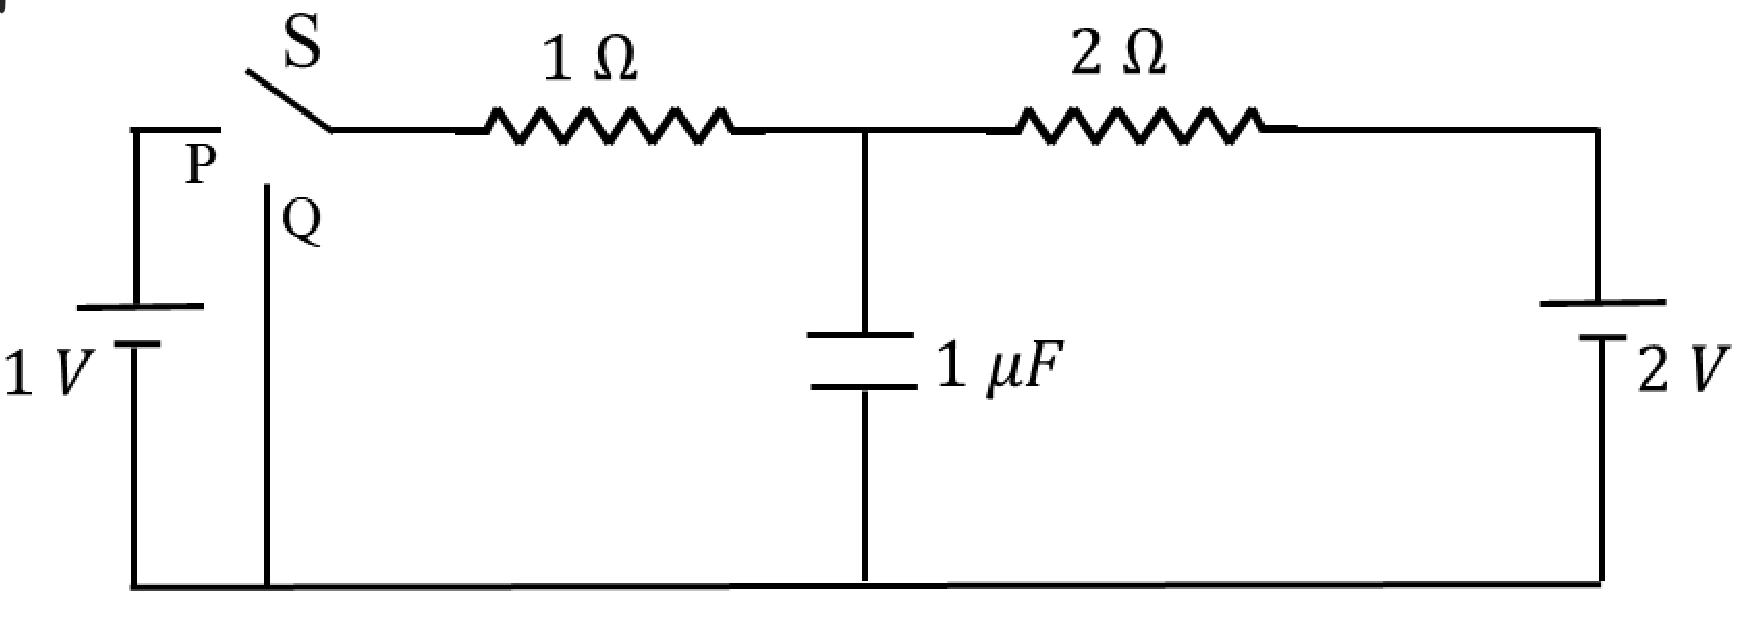
\includegraphics[width=\columnwidth]{figs/ckt.jpg}
			\caption{}
			\label{fig:ckt}
\end{figure}
\item Draw the circuit using latex-tikz.

\solution

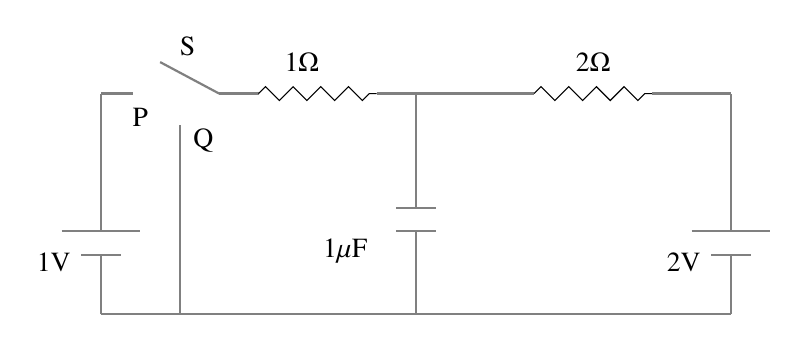
\begin{tikzpicture}
\draw[gray, thick] (0.75,1.2) -- (0.75,3.6); %Q
\draw[gray, thick] (0.5,4.4) -- (1.25,4); %S
\draw[gray, thick] (-0.25,4) -- (0.15,4); %P

\draw[gray, thick] (1.25,4) -- (1.75,4); %R_1 and R_2
\draw[decorate,decoration=zigzag] (1.75,4) -- (3.25,4);
\draw[gray, thick] (3.25,4) -- (5.25,4);
\draw[decorate,decoration=zigzag] (5.25,4) -- (6.75,4);
\draw[gray, thick] (6.75,4) -- (7.75,4);



\draw[gray, thick] (-0.25,1.2) -- (-0.25,1.95); %1V
\draw[gray, thick] (-0.25,2.25) -- (-0.25,4);
\draw[gray, thick] (-0.5,1.95) -- (0,1.95);
\draw[gray, thick] (-0.75,2.25) -- (0.25,2.25);

\draw[gray, thick] (7.75,1.2) -- (7.75,1.95); %2V
\draw[gray, thick] (7.5,1.95) -- (8,1.95);
\draw[gray, thick] (7.25,2.25) -- (8.25,2.25);
\draw[gray, thick] (7.75,2.25) -- (7.75,4);

\draw[gray, thick] (3.75,1.2) -- (3.75,2.25); %capacitor
\draw[gray, thick] (3.75,2.55) -- (3.75,4);
\draw[gray, thick] (3.5,2.25) -- (4,2.25);
\draw[gray, thick] (3.5,2.55) -- (4,2.55);

\draw[gray, thick] (-0.25,1.2) -- (7.75,1.2); %base

\node[] at (-0.85,1.85) {1V};
\node[] at (7.15,1.85) {2V};
\node[] at (2.85,2) {1$\mu$F};
\node[] at (0.25,3.7) {P};
\node[] at (0.85,4.6) {S};
\node[] at (1.05,3.4) {Q};
\node[] at (2.3,4.4) {1$\ohm$};
\node[] at (6,4.4) {2$\ohm$};
\end{tikzpicture}
\item Find $q_1$.

\solution
No current will pass through the capacitor, hence
\[i = \frac{2-1}{2+1} = \frac{1}{3}A\]
\[V_c = 2 - 2.i = \frac{4}{3}V\]
\[ q_1 = \frac{4}{3}\mu C\]
	\item Show that the Laplace transform of $u(t)$ is $\frac{1}{s}$ and find the ROC.

 \solution
 \[U(s)=\int_{-\infty}^{\infty}u(t)e^{-st}dt\]
 \[ = \int_{0}^{\infty}e^{-st}dt = \frac{1}{s}, \quad s>0\]
	\item Show that 
		\begin{align}
			e^{-at}u(t) \system{L} \frac{1}{s+a}, \quad a > 0
		\end{align}
		and find the ROC.
  
  \solution
  \[ = \int_{-\infty}^{\infty}u(t)e^{-at}e^{-st}dt\]
  \[ = \int_{0}^{\infty}e^{-(s+a)t}dt\]
  \[= \frac{1}{s+a}, \quad s+a>0 \]
\item Now consider the following resistive circuit transformed from 
			Fig. \ref{fig:ckt}
		\begin{figure}[!ht]
			\centering
			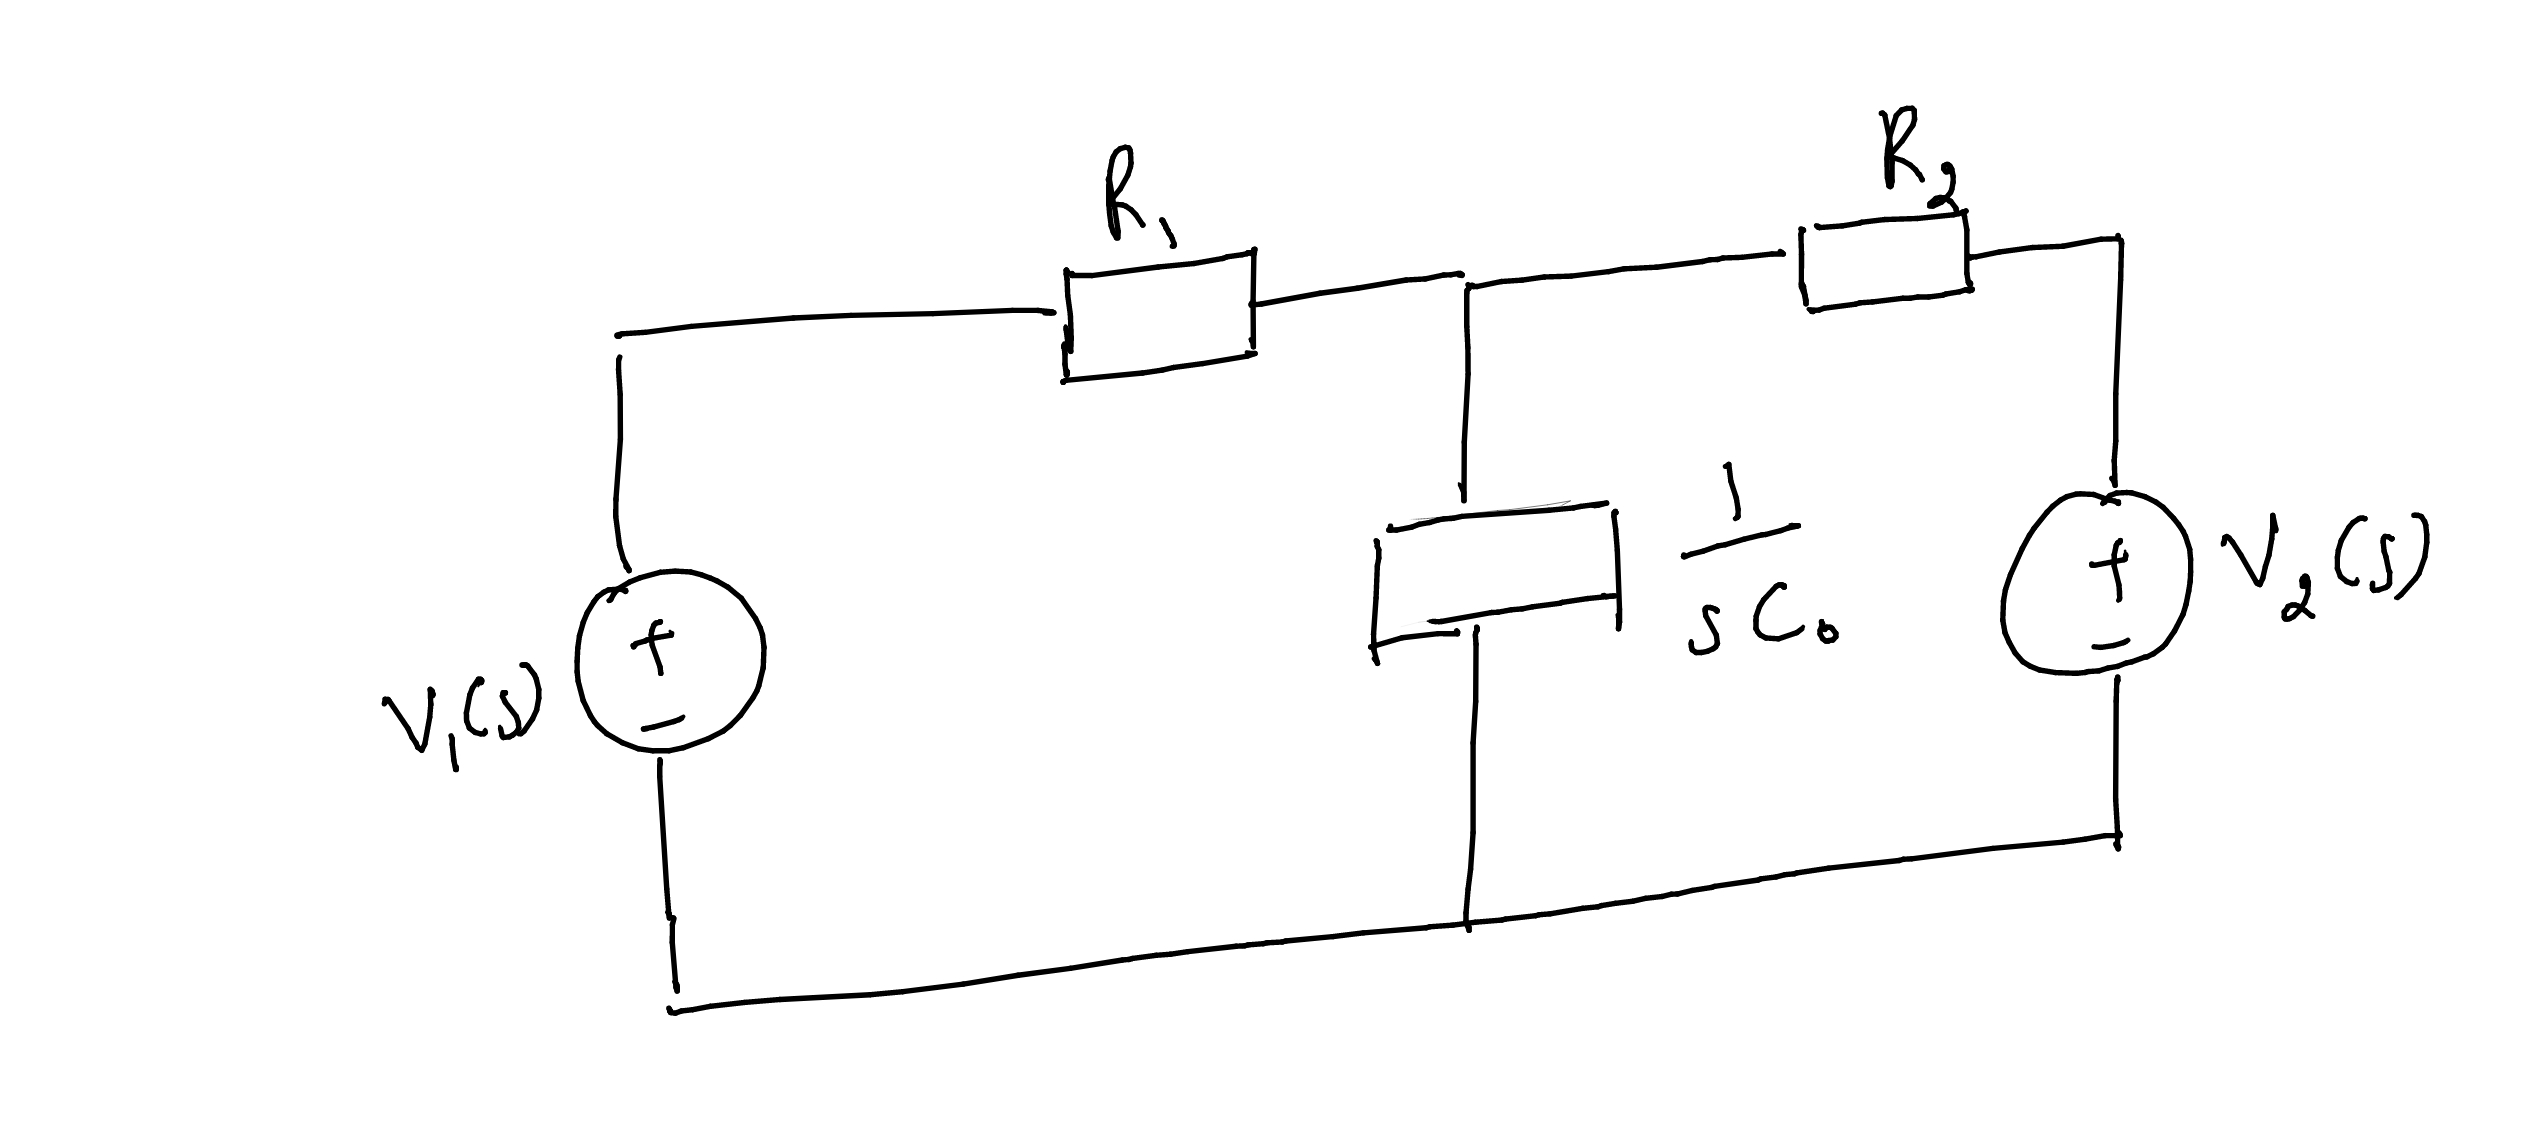
\includegraphics[width=\columnwidth]{figs/lap-ckt.jpg}
			\caption{}
			\label{fig:lap-ckt}
\end{figure}
		where 
		\begin{align}
			u(t) \system{L} V_1(s)
			\\
			2u(t) \system{L} V_2(s)
		\end{align}
		Find the voltage across the capacitor $V_{C_0}(s)$.
  \solution
  From Q2.4
  \[V_1(s) = \frac{1}{s} \quad V_2(s) = \frac{2}{s}\]
  \[\frac{V_1-V_C}{R_1} + \frac{V_2 - V_C}{R_2} - V_CsC = 0\]
  simplifying,
  \[\implies V_c(s)=\frac{2R_1 + R_2}{R_1 + R_2}\brak{\frac{1}{s} - \frac{1}{\frac{R_1 + R_2}{R_1R_2C}+s}}\]
	\item Find $v_{C_0}(t)$.  Plot using python.
 
 \solution
 Using the inverse Laplace transform from the obtained $V_c(s)$ we get,
 \[v_c(t) = \frac{2R_1 + R_2}{R_1 + R_2}u(t)\brak{1-e^{-\frac{R_1+R_2}{R_1R_2C}t}}\]
 \[R_1 = 1\ohm \quad R_2 = 2\ohm \quad C = 1\mu F\]
 \[v_c(t) = \frac{4}{3}u(t)\brak{1-e^{-1.5\times10^{6}t}}\]
 \begin{lstlisting}
     wget https://github.com/Galahad7377/EE3900/blob/main/cktsig/codes/2.7.py
 \end{lstlisting}
 \begin{figure}[!ht]
			\centering
			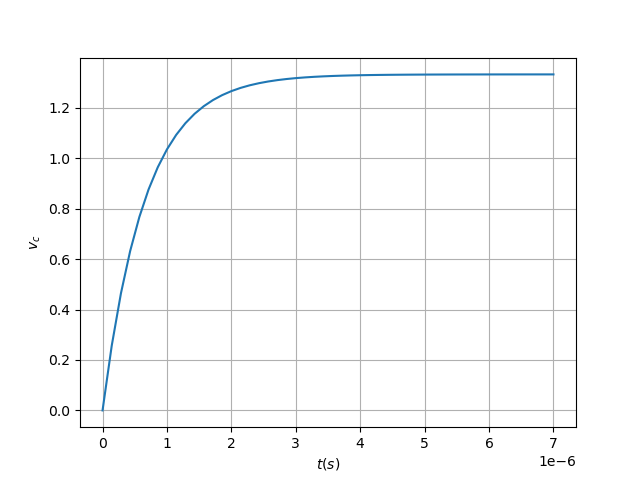
\includegraphics[width=\columnwidth]{figs/2.7.png}
			\caption{$v_c(t)$}
			\label{}
\end{figure}
	\item Verify your result using ngspice.

 \solution
 \begin{lstlisting}
     wget https://github.com/Galahad7377/EE3900/blob/main/cktsig/codes/2.8.cir
 \end{lstlisting}
 \begin{figure}[!ht]
			\centering
			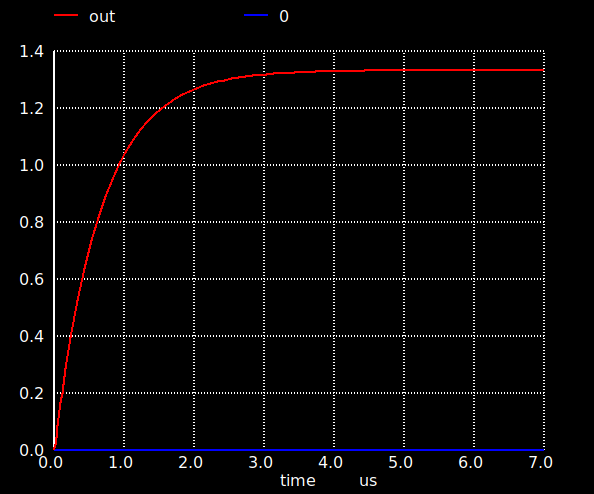
\includegraphics[width=\columnwidth]{figs/2.8.png}
			\caption{}
			\label{}
\end{figure}
	\item Obtain Fig. 
			\ref{fig:lap-ckt}
			using the equivalent differential equation.

   \solution
   \[\frac{dq}{dt} = \frac{V_1 - V_c}{R_1} +\frac{V_2 - V_c}{R_2}\]
   \[\frac{dq}{dt} = 1 - \frac{q}{C} + \frac{1}{2}\brak{2-\frac{q}{C}}\]
   simplifying and integrating,
   \[\int_0^{q_1} \frac{dq}{2-1.5q/C} = \int_0^tdt\]
   \[\ln{\frac{2-1.5q/C}{2} = 1.5\frac{t}{C}\]
   \[\implies q_1 = \frac{4}{3}\brak{1-e^{-1.5\times10^{6}t}}\times10^{-6}\]
   
\end{enumerate}

 \section{Initial Conditions}
\begin{enumerate}[label=\arabic*.,ref=\thesection.\theenumi]
\numberwithin{equation}{section}
\item Find $q_2$ in Fig. 
			\ref{fig:ckt}.

   
   \solution
   \[i=\frac{2}{1+2} = \frac{2}{3}A\]
   \[V_c = 2 - 2.i = \frac{2}{3}V\]
   \[\implies q_2 = CV_c = \frac{2}{3}\mu C\]
\item Draw the equivalent $s$-domain resistive circuit when S is switched to position Q.  Use variables $R_1, R_2, C_0$ for the passive elements.
Use latex-tikz.

\solution
\\

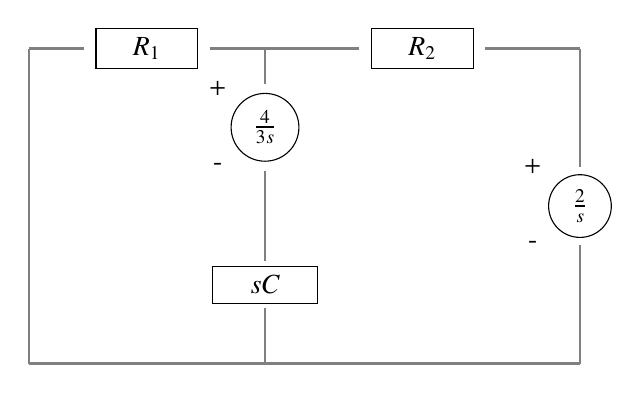
\begin{tikzpicture}

\draw[gray, thick] (1,0) -- (1,4); %Q
% \draw[gray, thick] (0.75,4.4) -- (1.5,4); %S
% \draw[gray, thick] (0,4) -- (0.6,4); %P

\draw[gray, thick] (1,4) -- (1.7,4); %R_1 and R_2
% \draw[decorate,decoration=zigzag] (2,4) -- (3.5,4);
\draw[gray, thick] (3.3,4) -- (5.2,4);
% \draw[decorate,decoration=zigzag] (5.5,4) -- (7,4);
\draw[gray, thick] (6.8,4) -- (8,4);

    \node[rectangle,draw] (r) at (2.5,4) {$\quad  R_1\quad$};
    \node[rectangle,draw] (r) at (6,4) {$\quad  R_2\quad$};
    \node[rectangle,draw] (r) at (4,1) {$\quad  sC\quad$};
    % \node[circle,draw] (r) at (4,3) {$V$};


% \draw[gray, thick] (0,0) -- (0,1.95); %1V
% \draw[gray, thick] (0,2.25) -- (0,4);
% \draw[gray, thick] (-0.25,1.95) -- (0.25,1.95);
% \draw[gray, thick] (-0.5,2.25) -- (0.5,2.25);

\draw[gray, thick] (8,0) -- (8,1.5); %2V
% \draw[gray, thick] (7.75,1.95) -- (8.25,1.95);
% \draw[gray, thick] (7.5,2.25) -- (8.5,2.25);
    \node[circle,draw] (r) at (4,3) {$\frac{4}{3s}$};
    \node[circle,draw] (r) at (8,2) {$\frac{2}{s}$};

\draw[gray, thick] (8,2.5) -- (8,4);

\draw[gray, thick] (4,0) -- (4,0.7); 
\draw[gray, thick] (4,2.45) -- (4,1.3); 
\draw[gray, thick] (4,3.55) -- (4,4);
% \draw[gray, thick] (3.75,1.95) -- (4.25,1.95);
% \draw[gray, thick] (3.75,2.25) -- (4.25,2.25);

\draw[gray, thick] (1,0) -- (8,0); %base

% \node[] at (-0.6,1.85) {1V};
\node[] at (3.4,2.5) {-};
\node[] at (3.4,3.5) {+};

\node[] at (7.4,1.5) {-};
\node[] at (7.4,2.5) {+};
% \node[] at (3.1,2) {$C_0$};
% \node[] at (0.5,3.7) {P};
% \node[] at (1.1,4.6) {S};
% \node[] at (2.55,4.4) {$R_1$};
% \node[] at (6.25,4.4) {$R_2$};
\end{tikzpicture}
\\
		\label{prob:init}
	
		\item $V_{C_0}(s)$ = ?  
  
  \solution
  \[\frac{V_C - 2/s}{R_2} + \frac{V_C}{R_1} + \brak{V_C - 4/3s}sC = 0\]
  \[V_C(s) = \frac{\frac{2}{sR_2} + \frac{4}{3}C}{\frac{1}{R_1} + \frac{2}{R_2} + sC}\]
	\item $v_{C_0}(t)$ = ? Plot using python.
 
 \solution Further simplifying,
 \[V_C(s) = \frac{4}{3}\brak{\frac{1}{\frac{R_1 + R_2}{R_1R_2C}+s}} + \frac{2R_1R_2}{R_2\brak{R_1+R_2}}\brak{\frac{1}{s} - \frac{1}{ \frac{R_1 + R_2}{R_1R_2C}+ s}}\]
 Using the inverse Laplace transform from the obtained Vc(s) we get,
 \[v_c(t) = \frac{4}{3}e^{{\frac{R_1 + R_2}{R_1R_2}\frac{t}{C}}} + \frac{2R_1R_2}{R_2\brak{R_1+R_2}}\brak{1 - e^{{ \frac{R_1 + R_2}{R_1R_2}\frac{t}{C}}}}\]
 \[R_1 = 1\ohm \quad R_2 = 2\ohm \quad C = 1\mu F\]
\[\implies v_c(t) = \frac{2}{3}u(t)\brak{1+e^{-1.5\times10^{6}t}}\]
\begin{lstlisting}
    wget https://github.com/Galahad7377/EE3900/blob/main/cktsig/codes/3.4.py
\end{lstlisting}
 \begin{figure}[!ht]
			\centering
			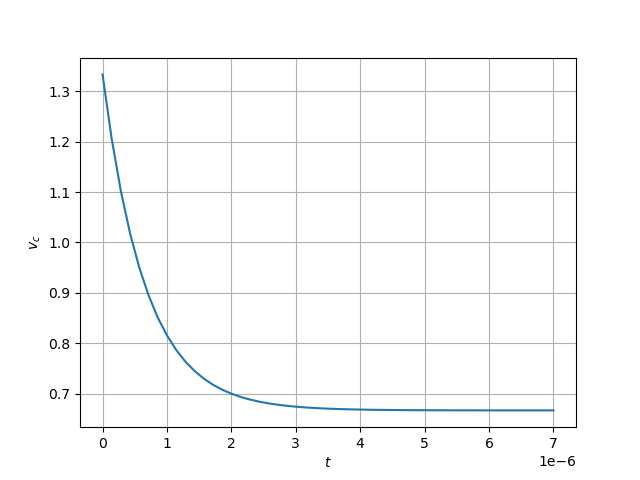
\includegraphics[width=\columnwidth]{figs/3.4.png}
			\caption{$v_c(t)$}
			\label{}
\end{figure}
	\item Verify your result using ngspice.

  \solution
 \begin{lstlisting}
     wget https://github.com/Galahad7377/EE3900/blob/main/cktsig/codes/3.5.cir
 \end{lstlisting}
 \begin{figure}[!ht]
			\centering
			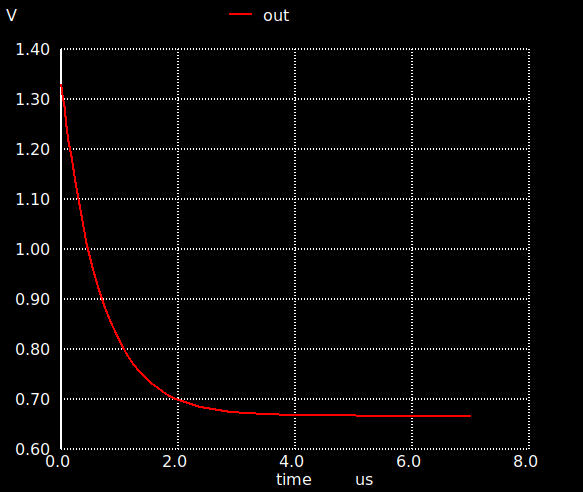
\includegraphics[width=\columnwidth]{figs/3.5.png}
			\caption{}
			\label{}
\end{figure}
	\item Find $v_{C_0}(0-), v_{C_0}(0+)$ and  $v_{C_0}(\infty) $. 
 
 \solution
 from section 2,
 \[v_c(0-) = \frac{4}{3}V\]
 from Q3.4
 \[v_c(0+) = \frac{4}{3}V\]
 \[v_c(\infty) = \frac{2}{3}V\]
	\item Obtain the Fig.  in problem 
		\ref{prob:init}
			using the equivalent differential equation.

   \solution
   \[\frac{dq}{dt} = \frac{2-V_C}{2} - V_C\]
   simplifying and integrating,
   \[\int_{4/3\mu C}^q \frac{dq}{2-3q/C} = 2\int_0^tdt\]
   \[\ln{\frac{2-3q/C}{-2}} = -1.5\frac{t}{C}\]
   \[q = \frac{2}{3}\brak{1+e^{-1.5\times10^{6}t}}\times10^{-6}\]


	\end{enumerate}

\end{document}